\documentclass{article}
%\usepackage[a4paper,top=0.75in, bottom=0.75in, left=1in, right=1in,footskip=0.2in]{geometry}
\usepackage{fullpage}
%-----------------Hyperlink Packages--------------------
\usepackage{hyperref}
\hypersetup{
	 colorlinks   = true,
     citecolor    = black,
     linkcolor    = black,
     urlcolor     = black
}
%-----------------Figure Packages--------------------
\usepackage{graphicx}                       % For figures
%\usepackage{epsfig} % for postscript graphics files
%------------------Math Packages------------------------
\usepackage{amssymb,amsmath}
\usepackage{textcomp}
\usepackage{mdwmath}
\usepackage{mdwtab}
\usepackage{eqparbox}
%------------------Table Packages-----------------------
\usepackage{rotating}                     % Used to rotate tables
\usepackage{array}                        % Fixed column widths for tables
%-----------------Algorithm Packages--------------------
\usepackage{listings}                     % Source code
\usepackage{algorithm}                    % Pseudo Code
\usepackage{algpseudocode}
%---------------------------------------------------------

%opening

\begin{document}

\title{
Data Mining Course Project \\
Parallel Random Forest
}
\author {
	Computer Application Class 2, 12330402\\
	Qiuyi Zhang (\href{mailto:joyeec9h3@gmail.com}{joyeec9h3@gmail.com})
}
\date{\today}

\maketitle
\tableofcontents


\section{Problem Description}

The dataset contains 6238 records for training and 1559 records for testing. Each record has 617 features and a label ranging in $[0, 25]$. Given this dataset, the goal is to train a random forest to predict the labels for the test set as precisely as possible.

\section{Algorithms}

For this project I implemented a random forest(with parallelism support) consisting of C4.5 decision trees built with Gini impurity.

\subsection{Decision Tree}

\subsubsection{Building Decision Trees}

The algorithm for building the decision tree is described in Algorithm~\ref{alg:dt}.

For simplicity, the trees are built recursively.

\begin{algorithm}[H]
\centering
\caption{Decision tree}
\label{alg:dt}
  \begin{algorithmic}[1]
    \Function{DecisionTree.fit}{$data$, $attributes$}
        \If{$data$ is empty}
        	\State \Return an empty node
        \EndIf

        \State $gain_{best}$ = 0.0, $attr_{best}$ = 0, $value_{best}$ = 0.0
        \State $set1_{best}$ = $\{\}$, $set2_{best}$ = $\{\}$

		\If{$data.size > MIN\_NODE\_SIZE$}
		    \For{each attribute $a$ in $attributes$}
			    \State Sort $data$ by their values of $a$, $threshold$ = the midpoint of the sorted $data$
	    		\State Divide $data$ by $threshold$ into $set1$, $set2$
	    		\State Calculate the information gain of spliting $data$ into $set1$ and $set2$
	    		\If{The new information gain $> gain_{best}$}
	    			\State Update $gain_{best}$, $attr_{best}$, $value_{best}$, $set1_{best}$, $set2_{best}$
	    		\EndIf
		    \EndFor
		\EndIf
	    \If{$attributes$ is not empty and $gain_{best} \neq 0.0$}
	    	\State remove $attr_{best}$ from $attributes$
	    	\State $this.left =$ \Call{DecisionTree.fit}{$set1_{best}$, $attributes$}
	    	\State $this.right =$ \Call{DecisionTree.fit}{$set1_{best}$, $attributes$}
			\State $this.attr = attr_{best}$
			\State $this.threshold = value_{best}$
			\State $this.cound = data.size$
			\State \Return $this$
      	\Else
      		\State Create a counter for labels in $data$
      		\State $this.leaf = counter$
      		\State \Return $this$
      	\EndIf
    \EndFunction
  \end{algorithmic}
\end{algorithm}

\begin{description}
\item Remark 1. \hfill \\
Suppose $i \in \{1, 2, ..., m\}$, and let $f_i$ be the fraction of items labeled with value $i$ in the set, the \textit{Gini impurity} for a set of items is defined as:

$$I_{G}(f) = \sum_{i=1}^{m} f_i (1-f_i) = \sum_{i=1}^{m} (f_i - {f_i}^2) = \sum_{i=1}^m f_i - \sum_{i=1}^{m} {f_i}^2 = 1 - \sum^{m}_{i=1} {f_i}^{2}$$


\item Remark 2.\hfill \\
When a data set $D$ with goal attribute $V$ is split into subsets $D_k$ using attribute $A$, each with $n_k$ records, the \textit{information gain} is defined as:

$$
Gain(A) = H(V, D) - Remainder(A)
$$

where

$$
Remainder(A) = \sum_k P(n_k) H(V, D_k)
$$

$P(n_k)$ is the proportion of $E_k$ in $D$.
\end{description}

\subsubsection{Use Decision Trees for Prediction}

The algorithm for predicting a label with a set of observations for the features are shown in Algorithm~\ref{alg:predictdt}. It's also recursive, therefore rather intuitive.

\begin{algorithm}[H]
	\centering
	\caption{Prediction using Decision Trees}
	\label{alg:predictdt}
	\begin{algorithmic}[1]
		\Function{DecisionTree.predict}{$this$, $observation$}
		\If{$this.leaves$ is a counter}
		\State\Return The most frequent item in $tree.leaves$
		\EndIf

		\State $value$ = $observation[this.attr]$
		\If{$value < this.threshold$}
		\State \Return \Call{DecisionTree.predict}{$this.left$, $observation$}
		\Else
		\State \Return \Call{DecisionTree.predict}{$tree.right$, $observation$}
		\EndIf
		\EndFunction
	\end{algorithmic}
\end{algorithm}

\subsection{Random Forest}

\subsubsection{Building Random Forest}

The algorithm for building a random forest out of a set of decision trees is described in Algorithm~\ref{alg:rf}. Notice that the sampling of records are without replacement, and the sampling of features are with replacement.

\begin{algorithm}[H]
\centering
\caption{Building a Random Forest}
\label{alg:rf}
  \begin{algorithmic}[1]
    \Function{RandomForest.fit}{$data$, $numTrees$, $numFeatures$, $numSampleCoeff$}
	    \State Sample $numSampleCoeff \times data.size$ records(without replacement) from $data$ as the $bootstrap$
	    \For{each $tree$ in this forest}
		    \State Sample $numFeatures$ attributes(with replacement) from the attribute set as $attributes$
		    \State $tree$ = \Call{$DecisionTree.fit$}{$bootstrap$, $attributes$}
	    \EndFor
    \EndFunction
  \end{algorithmic}
\end{algorithm}

\subsection{Use the Random Forest for Prediction}

The algorithm for classifying an observation is described in Algorithm~\ref{alg:predictrf}. It uses the most popular result from the predictions produced by the trees.

\begin{algorithm}[H]
	\centering
	\caption{Prediction using a Random Forest}
	\label{alg:predictrf}
	\begin{algorithmic}[1]
		\Function{RandomForest.predict}{$observations$}
			\State $result = []$ 

			\For{each $row$ with index $i$ in $observations$}
				\State Create a new $counter$
				\For {each $tree$ in the forest}
					\State $counter.add$\Call{$tree$.predict}{$row$}
				\EndFor
				\State $result[i]$ = the most frequent item in $counter$
			\EndFor

			\State \Return $result$
		\EndFunction
	\end{algorithmic}
\end{algorithm}

\section{Implementation}

\subsection{Parallelism}

The random forest can be easily parallelized since the training and classifying done in each tree can be completely separated. To build a parallel implementation, there are many options available: multi-threading, MPI, Map-reduce(Hadoop), Spark, etc. Because the computational resources I have are limited, I chose threads to parallelize the implementation. Using OpenMP, which is built in most compilers nowadays, it's fairly trivial to parallelize the for loops in the random forest(a few simple \texttt{\#pragma} directives will suffice).

On a machine with Intel i7-4710HQ@2.5GHz(which has 4 cores and 8 hyperthreads) and 8G RAM, it takes the program(built with VS2013) about 170s to build a random forest with 1000 trees when multi-threading is not enabled(see Figure~\ref{fig:single}), and  about 40s when multi-threading is enabled(see Figure~\ref{fig:multi}). In the first case, only 25\% of the CPU can be utilized while in the second case, 100\% of the CPU is utilized.

\begin{figure}[]
	\centering
	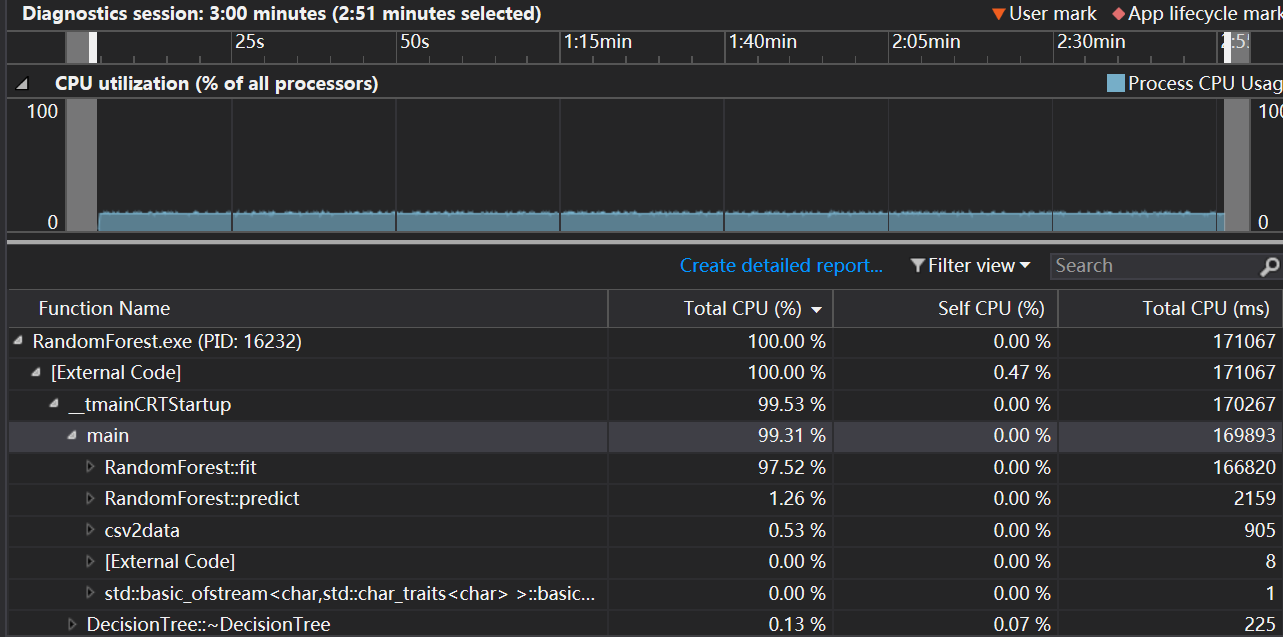
\includegraphics[width=\linewidth]{single.png}
	\caption{Performance analysis of the implementation without multi-threading}
	\label{fig:single}
\end{figure}

\begin{figure}[]
	\centering
	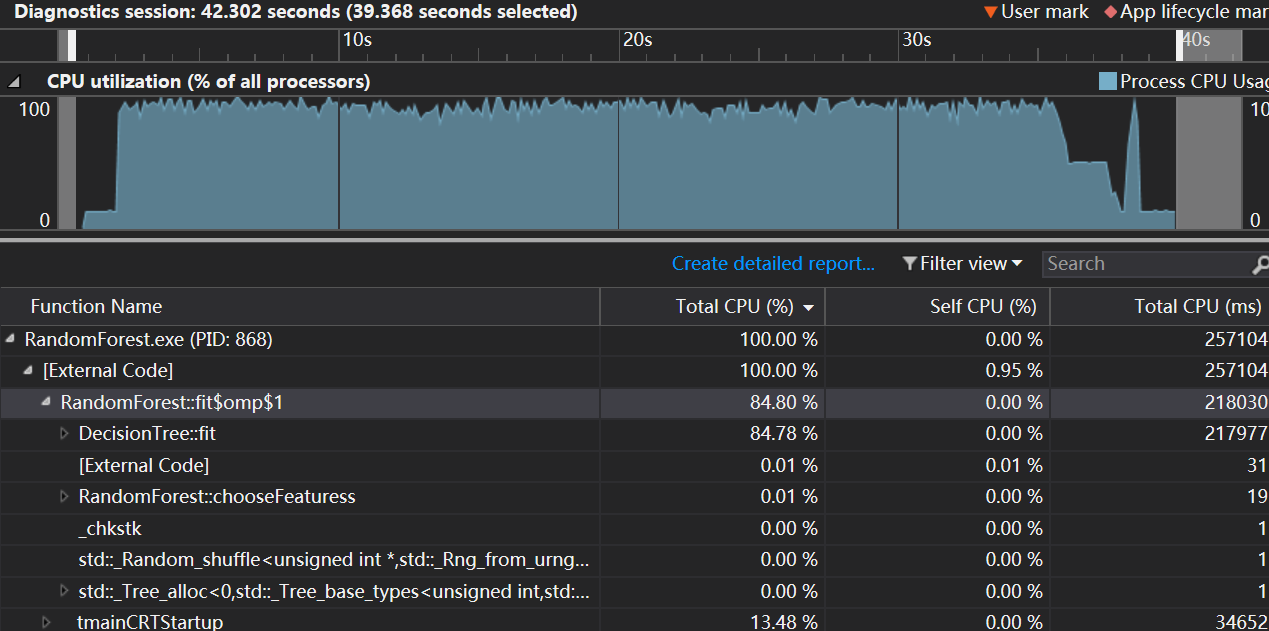
\includegraphics[width=\linewidth]{multi.png}
	\caption{Performance analysis of the implementation with multi-threading}
	\label{fig:multi}
\end{figure}

\subsection{Cross-platform}

This implementation was originally developed with Visual Studio 2013. By using Premake, it can also be built with MinGW under Windows, or with g++/clang++ under Linux. See README.md for instructions on how to build it on other platforms.

\section{Experiment Results}

For applications of random forests, there are some critical parameters that needs to be tuned:

\begin{enumerate}
	\item \textbf{Number of trees in the forest}. Generally speaking, the more trees in the forest, the better the predictions will be.
	\item \textbf{Number of sampled features}. A rule of thumb for it is $\log_2n$ where $n$ is the number of features in the dataset.
	\item \textbf{Minimum size of tree nodes}. The minimum number of samples required to split a node.
	\item \textbf{Size of the bootstrap}. Generally speaking, if the size of the bootstrap is the same as the size of the training set(which means some rows could be chosen multiple times while some would be left out), the random forest will typically provide near-optimal performance.
	\item And more...
\end{enumerate}

For this project, I used 1000 trees in the forest, $\log_2n$ features, set the minimum size of tree nodes to be 2, and use a bootstrap the same size as the training set. This configuration gives a $96.144\%$ precision when tested on the Kaggle platform, see Figure~\ref{fig:kaggle}.

\begin{figure}[]
	\centering
	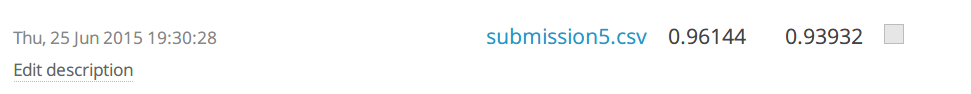
\includegraphics[width=\linewidth]{kaggle.png}
	\caption{Score on Kaggle}
	\label{fig:kaggle}
\end{figure}

\end{document}
